\section{Analýza frameworků}

V~této části práce se zabýváme analýzou frameworků Angular, React, Svelte a~Vue. Nejdříve analyzujeme každý framework samostatně. 
Zaměříme se především na klíčové koncepty frameworků, stavební bloky, správu stavů, předávání vlastností. 
Dále rozebereme životní cykly, state management, routování a~ekosystém jednolivých technologií. 
Kapitolu zakončíme porovnáním analyzovaných frameworků.

Výběr porovnávaných technologií byl proveden na základě analýzy výsledků z~Developer Survey 2023 od Stack Overflow. 
Rozhodující byla sekce \emph{Web frameworks and technologies}, ve které byly hodnoceny webové technologie dle jejich žádanosti na trhu a~obdivem mezi vývojářskou komunitou. 
Tato strategie zajistila, že vybrané frameworky odpovídají současným trendům a~potřebám webového vývoje, ale také vycházejí z~uznání a~podpory komunity.\cite{stackoverflow, developersurvey}

\subsection{Angular}

Angular byl původně interní JavaScriptový framework společnosti Google. 
Dle oficiální dokumentace \cite{angulario} je Angular kompletní platforma, určená k~vývoji webových aplikací. 
Framework je postaven na principu komponent, jež tvoří základní stavební jednotku aplikace. 
Součástí frameworku jsou knihovny, které jsou velmi dobře integrovatelné a~usnadňují práci s~různými částmi aplikace. 
Dále také nástroje, které vývojářům usnadňují vývoj, testování či aktualizaci kódu.\cite{angulario,learningangular}

\begin{figure}[htb]
	\centering
		
\includegraphics[width=.5\textwidth]{images/angular-logo.png}
	\caption[Angular logo]{Angular logo \cite{angulardev}}
	\label{fig:angularlogo}
\end{figure}

První verze Angularu byla vydána v~roce 2012 a byla nazvána AngularJS. 
Později v~roce~2016, po kolaboraci se společností Microsoft, Google vydal novou verzi, o~které mluvíme jako o~Angular~2. 
Druhá verze byla kompletně přepsána z~JavaScriptu do jazyku TypeScript. 
Součástí frameworku je i~knihovna pro práci s~asynchronními událostmi -- RxJS \cite{rxjslibrary}, kterou vývojáři využívají k~reaktivnímu programování. 
Angular se samozřejmě neustále vyvíjí a~v~současné době můžeme pracovat s~verzí~17.\cite{angulardev,learningangular}

Díky robustnosti a~velikosti frameworku je Angular vhodnější pro větší aplikace, které vyžadují mnoho funkcí a~komplexních struktur. 
V~poslední době framework spíše ztrácí na popularitě, stále jej však používá mnoho společností včetně Google.\cite{learningangular}

\subsubsection{Komponenty}

Hlavní bloky kódu Angularu tvoří komponenty. Komponenta je OOP třída definovaná v~TypeScript souboru ve formátu nazev-tridy.component.ts. 
Komponentu nastavujeme pomocí dekorátoru @Component, v~němž definujeme selektor (HTML značku komponenty), šablonu, případně kaskádové styly a~použité API. 
Komponenta se může skládat z~dalších částí: šablony, kaskádových stylů a~testovacích scénářů definovaných v~samostatném souboru. 
Tyto soubory jsou nepovinné, obvykle jsou však žádoucí a~vedou k~lepší organizaci kódu. 

Původní komponenty byly tvořeny pomocí modulů (NgModules), které obsahovaly deklarace komponent, direktiv a~služeb. 
Od verze~14 je možné využít standalone API, které umožňuje vytvářet komponenty bez nutnosti tvoření a~registrace modulů v~jiných souborech, a~díky tomu je kód kratší. 
V~dekorátoru @Component pak je třeba importovat všechny potřebné závislosti -- direktivy, služby či jiné komponenty.\cite{angulardev,learningangular}

V~šabloně vykreslíme hodnoty pomocí dvojitých závorek, které obsahují název proměnné. K~podmíněnému zobrazení komponent/elementu slouží bloky @if, @else if, @else. 
Pro iteraci přes pole hodnot slouží blok @for.\cite{angulardev}

\begin{prog}
import \{ Component \} from '@angular/core';

@Component(\{
  selector: 'my-component',
  standalone: true,
  template: `
    <div>\{\{ content \}\}</div>
  `,
  styles: ['div \{ background-color: red; \}']
\})
export class MyComponent \{
  content = 'nějaký-obsah';
\}
\end{prog}

\subsubsection{Správa stavů}

K~vytvoření stavů v~Angularu využijeme vlastnosti třídy (class fields). Vlastnosti mohou být veřejné (public), protected (chráněné) nebo soukromé (private). 
V~případě, že viditelnost nespecifikujeme, je vlastnost veřejná. Soukromé vlastnosti jsou viditelné pouze v~rámci třídy, chráněné v~rámci třídy a~šablony. 
Veřejné vlastnosti jsou viditelné odkudkoli.\cite{angulardev,learningangular}

Pro aktualizaci stavů využijeme přiřazení nové hodnoty do vlastnosti, k~níž přistoupíme pomocí klíčového slova this.\cite{angulardev}

\begin{prog}
import \{ Component \} from '@angular/core';

@Component(\{
  selector: 'my-component',
  standalone: true,
  template: `
    <button (click)="increment()">
      Klikli jste na tlačítko \{\{ count \}\}x.
    </button>
  `,
\})
export class MyComponent \{
  protected count = 0;

  protected increment(): void \{
    this.count++;
  \}
\}
\end{prog}

Počínaje verzí~16 můžeme používat také nestabilní verzi signálů (Angular Signals), přičemž se jedná o~systém, který mnohem efektivněji sleduje využití stavů v~rámci aplikace. 
Signály pak umožňují efektivnější a~optimalizovanější aktualizace DOM. 

\begin{prog}
import \{ Component, signal \} from '@angular/core';

@Component(\{
  selector: 'my-component',
  standalone: true,
  template: `
    <button (click)="increment()">
      Klikli jste na tlačítko \{\{ count() \}\}x.
    </button>
  `,
\})
export class MyComponent \{
  protected count = signal(0);

  protected increment(): void \{
    this.count.update((value) => value + 1);
  \}
\}
\end{prog}

Od verze~17 jsou signály stabilní součástí Angularu, na druhou stranu předávání a~modely signálů zatím stabilní nejsou. 
Proto v~této práci budeme využívat klasické hodnoty stavů.\cite{angulardev}

\subsubsection{Předávání vlastností}

Předávat vlastnosti či jiné hodnoty je možné pomocí vstupního dekorátoru @Input a~výstupního dekorátoru @Output. 
V~rámci šablony danou hodnotu předáme do vnořené komponenty skrze název vstupu v~hranatých závorkách.   
Ve vnořené komponentě využijeme dekorátor @Input, sloužící k~získání hodnot z~rodičovské komponenty. K~předaným hodnotám není možné přistupovat v~rámci konstruktoru. 

K~předání hodnoty z~vnořené komponenty nejprve přidáme vnořené komponentě název výstupu v~kulatých závorkách a~obslužnou metodu, která se vykoná po předání vlastnosti. 
Posléze definujeme @Output ve vnořené komponentě, na němž zavoláme metodu emit(), která přes argument metody umožňuje předání (vypublikování) hodnot z~vnořené do rodičovské komponenty.\cite{angulardev,learningangular}

\begin{prog}
import \{ CommonModule \} from '@angular/common';
import \{ Component, Input, Output, EventEmitter \} from '@angular/core';

@Component(\{
  selector: 'parent-component',
  standalone: true,
  imports: [ChildComponent],
  template: `
    <child-component 
      [color]="someProps.color" 
      (colorClicked)="handleColorClicked(\$event)" 
    />
    <p>\{\{ colorClickedText \}\}</p>
  `,
\})
export class ParentComponent \{
  protected someProps = \{ color: 'cervena' \};
  protected colorClickedText = 'Na název barvy jste zatím neklikli.';

  protected handleColorClicked(clickCount: number): void \{
    this.colorClickedText = `Na název barvy 
      v ChildComponent jste klikli: \$\{clickCount\}x`;
  \}
\}

@Component(\{
  selector: 'child-component',
  standalone: true,
  imports: [CommonModule],
  template: `<p [ngClass]="color" (click)="handleClick()">\{\{ color \}\}</p>`,
\})
export class ChildComponent \{
  private clickCount = 0;

  @Input() color = 'Žádná barva nebyla specifikována.';
  @Output() colorClicked = new EventEmitter<number>();

  protected handleClick(): void \{
    this.clickCount++;
    this.colorClicked.emit(this.clickCount);
  \}
\}
\end{prog}

\subsubsection{Služby, direktivy, roury}

Angular disponuje pestrou škálou možností, jak sdílet bloky kódu či logiku mezi různými částmi aplikace. Služby, direktivy, nebo také roury tvoříme pomocí JavaScriptových tříd. 
Služby (services) umožňují znovupoužití určité části kódu např.~v~rámci více komponent. 
Služby obvykle používáme ke komunikaci s~HTTP endpointy, sdílíme v~nich stavy více komponent a~využíváme je k~transformacím.\cite{angulardev,learningangular}

\begin{prog}
import \{ Injectable \} from '@angular/core';
  
@Injectable(\{ providedIn: 'root' \})
export class DataService \{
  private data = 'Initial data';

  getCurrentData(): string \{
    return this.data;
  \}
      
  setNewData(newData: string): void \{
    this.data = newData;
  \}
\}
\end{prog}

Direktivy (directives), ať už zabudované či vlastní, slouží k~obohacení HTML elementů o~různé funkce (dynamické atributy, CSS třídy) nebo manipulaci s~DOM elementy. 
Roury (pipes) umožňují trasformaci hodnot v~šabloně.\cite{angulardev,angulario}

\begin{prog}
import \{ Component, Pipe, PipeTransform \} from '@angular/core';

@Pipe(\{ name: 'czechDate', standalone: true \})
export class CzechDateFormatPipe implements PipeTransform \{
  transform(value: Date): string \{
    return value.toLocaleDateString('cs-CZ');
  \}
\}

@Component(\{
  selector: 'my-component',
  standalone: true,
  imports: [CzechDateFormatPipe],
  template: `<p>\{\{ today | czechDate\}\}</p>`,
\})
export class MyComponent \{
  protected today = ;
\}
\end{prog}

\subsubsection{Životní cyklus}

Životním cyklem komponenty rozumíme sekvenci kroků, které se vykonají mezi vytvořením a~zničením komponenty. 
Životní cyklus může být rozdělen do čtyř částí: vytvoření, aktualizace, vykreslení a~zničení. 

První metoda, která se spouští při vytvoření komponenty, je konstruktor. 
Poté můžeme využít metody ngOnInit, ngOnChanges, ngDoCheck, ngAfterViewInit, ngAfterContentInit, ngAfterViewChecked, ngAfterContentChecked, jež se spouští v~různých fázích aktualizace (detekce). 
Nedávno byly přidány také metody, které se volají po vykreslení komponenty -- afterNextRender a~afterRender. 
V~neposlední řadě metoda ngOnDestroy je volána při zničení komponenty.\cite{angulardev,learningangular}

\begin{figure}[htb]
	\centering
		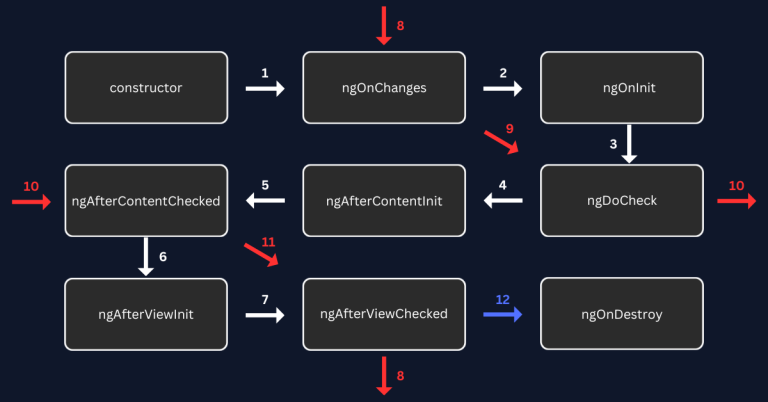
\includegraphics[width=.85\textwidth]{images/angularlifecycle.png}
	\caption[Životní cyklus Angularu]{Životní cyklus Angularu \cite{angularlifecycle}}
	\label{fig:angularlifecycle}
\end{figure}

\subsubsection{State management}

K~základní práci se stavy slouží vlastnosti třídy, které inicializujeme JavaScriptovou hodnotou. 
Do budoucna můžeme počítat s~lepší podporou signálů, které aktualizují DOM efektivněji a~rychleji. 
Pokročilejší způsob sdílení stavů v~rámci aplikace spočívá ve využití služeb, v~nichž uložíme stavy a~následně je sdílíme mezi komponentami.\cite{angulardev}

Pro reaktivní či asynchronní operace, nebo obecně složitější funkcionality, využijeme balíček RxJS, který je již součástí Angularu. 
RxJS poskytuje datový typ Observable, který reprezentuje data, jež se mohou měnit v~čase.\cite{angulario,rxjslibrary}

V~případě, že potřebujeme sdílet stavy globálně (mezi různými částmi aplikace), můžeme využít knihovnu NgRx, která je inspirována knihovnou Redux.\cite{angularstatemanagement,ngrxlib}

\subsubsection{Routování}

Angular poskytuje vestavěný systém routování -- konkrétně balíček @angular/router, který na straně klienta umožňuje přepínat mezi různými částmi aplikace. 
Klasické webové stránky při změně URL pokaždé žádají o~nové dokumenty. Routování na straně klienta může provést aktualizaci stránky bez dalších duplikátních dotazů. 
Při vyžádání dané cesty pak vykreslíme požadovaný obsah a~požádáme pouze o~data potřebná k~vykreslení. 
Získáme tak rychlejší uživatelskou zkušenost, jelikož prohlížeč nevyžaduje nové dokumenty a~nemusí vyhodnocovat kaskádové styly či JavaScript.

Abychom zaregistrovali cesty aplikace pomocí knihovny @angular/router, poskytneme samotný router pomocí funkce provideRouter do aplikačního nastavení. 
Routeru následně předáme pole cest aplikace. Jednotlivé obsahy stránek, které se mají zobrazit, vykreslíme pomocí elementu router-outlet.\cite{angulardev,learningangular}

\subsubsection{Ekosystém}

Angular je komplexní framework, v~němž jsou obsaženy základní balíčky všeho druhu potřebné pro vývoj webových aplikací. 
Framework se stále vyvíjí a~jeho ekosystém se neustále rozrůstá, a~to i~přes velikost projektu. 
Angular nabízí rozsáhlou kolekci balíčků třetích stran, které vývojáři využívají pro usnadnění práce s~různými částmi aplikace. 
Nechybí ani balíček @angular/cli, jenž usnadňuje vývoj aplikace, testování, aktualizaci kódu i~nasazení.\cite{angulardev,learningangular}
\subsection{React}

Pod pojmem React rozumíme open-source JavaScript framework, který vytvořila a~dále rozvíjí společnost Meta (dříve Facebook). 
Podle \cite{reactbanks} jde spíše o~knihovnu funkcí, než-li o~komplexní nástroj pro tvorbu webových aplikací (framework). 
Tato technologie se používá pro vývoj interaktivních uživatelských rozhraní a~webových aplikací.\cite{reacthubspot}

\begin{figure}[htb]
	\centering
		
\includegraphics[width=.3\textwidth]{images/react-logo.png}
	\caption[React logo]{React logo \cite{react}}
	\label{fig:reactlogo}
\end{figure}

První kořeny Reactu sahají až do roku 2010, kdy tehdejší společnost Facebook přidala novou technologii XHP do PHP. 
Jde o~možnost znovu použít určitý blok kódu, stejného principu posléze využívá i~React. Následně Jordan Walke vytvořil FaxJS, jenž byl prvním prototypem Reactu.
O~rok později byl přejmenován na React a~začal jej využívat Facebook. 
V~roce 2013 byl na konferenci JS ConfUS představen široké veřejnosti a~stal se open-source.

Od roku 2014 vývojáři představují nespočet vylepšení samotné knihovny, stejně jako spoustu rozšíření pro zlepšení vývojových procesů. 
Kolem roku 2015 postupně React nabývá na popularitě i~celkové stabilitě. Následně je představen také React Native, což je framework pro vývoj nativních aplikací.
React používá široká škála společností, od malých startupů až po velké nadnárodní korporace. 
Z~těch největších jde například o~Metu, Uber, Twitter a~Airbnb.\cite{reactbanks,reactrisingstack}

\subsubsection{Komponenty}

Hlavním stavebním kamenem Reactu jsou komponenty, jež představují nezávislé, vnořitelné a~opakovaně použitelné bloky kódu. 
Komponentu v~Reactu tvoří JavaScript funkce a~HTML šablona. Validně seskládané komponenty poté tvoří webovou aplikaci.
V~Reactu se můžeme setkat s~funkčními a~třídními komponentami. Vytváření třídních komponent je na ústupu a~oficiální dokumentace je rovněž nedoporučuje. 
Výstup komponent tvoří elementy ve formě JSX. Tyto elementy obsahují informace o~vzhledu a~funkcionalitě dané komponenty.

Pro komunikaci mezi komponentami se používá předávání vlastností (props), přes které je možné předávat hodnoty jakýchkoli datových typů. 
Vlastnost vnořené komponentě předáme stejně jako atribut HTML elementu. 
Pro předání hodnoty do rodičovské komponenty slouží tzv. callback funkce, které se volají ve vnořené komponentě, ale modifikují vlastnosti rodičovské komponenty.\cite{reactbanks,react}

\begin{prog}
import React from 'react';

function ParentComponent() \{
  const someProps = \{color: 'cervena'\};

  return (
    <div>
      <ChildComponent color=\{'cervena'\} />
      <ChildComponent color=\{someProps.color\} />
      <ChildComponent \{...someProps\} />
    </div>
  );
\}

function ChildComponent(\{color\}) \{
  return (
    <div className=\{color\}></div>
  );
\}
\end{prog}

\subsubsection{JSX}

Název JSX kombinuje zkratku jazyka JavaScript -- JS a~počáteční písmeno ze zkratky XML. 
Konkrétně jde o~syntaktické rozšíření, které vývojářům umožňuje tvořit React elementy pomocí hypertextového značkovacího jazyku přímo v~JavaScriptu. 
V~rámci JSX pak je možné dynamicky vykreslovat obsah na základě logiky definované pomocí JS hodnot.
Při kompilaci se JSX překládá do JavaScriptu pomocí nástroje Babel.\cite{reactbanks,react}

\begin{prog}
import React from 'react';
import ChildComponent from './ChildComponent';

function MyComponent() \{
  const loaded = true;

  return (
    <div>
      \{loaded ? 
        <ChildComponent color=\{'cervena'\} width=\{100\} heigth=\{100\} /> 
        : 'Načítání ...'\}
    </div>
  );
\}
\end{prog}

\subsubsection{Správa stavů}

Stav lze definovat jako lokální vnitřní vlastnost či proměnnou dané komponenty, jež představuje základní mechanismus pro uchovávání a~aktualizaci dat. 
Pro aktualizaci komponenty je tedy nutné stav změnit. React pak na tuto skutečnost zareaguje a~vyvolá tzv. re-render neboli překreslení komponenty s~novými daty.

Za účelem ukládání stavu se využívá hook (funkce) useState. Ten poskytuje stavovou proměnnou, přes kterou se dostaneme k~aktuálnímu stavu. 
Dále useState poskytuje state setter funkci, díky které můžeme stav aktualizovat. Jediný argument useState definuje počáteční hodnotu daného stavu.\cite{reactitnetwork,react}

\begin{prog}
import React, \{ useState \} from 'react';

function App() \{
  const [count, setCount] = useState(0);

  return (
    <button onClick=\{() => setCount(count + 1)\}>
      Klikli jste na tlačítko \{count\}x.
    </button>
  );
\}
\end{prog}

\subsubsection{Hooky}

Specifickou funkcionalitou pro React jsou tzv. hooky, které byly do Reactu přidány až ve verzi 16.8.0.\cite{reactgithub} 
Hook je definován jako funkce, která obohacuje komponenty pomocí předdefinovaných funkcionalit. Jedním z~nejpoužívanejších hooků je useState. 
Vývojáři mohou používat již zabudované hooky, nebo si vytvářet své vlastní s~pomocí předdefinovaných hooků. 
Mezi zabudované hooky patří např. useEffect, useMemo, useCallback, useRef, useContext.\cite{react}

\begin{prog}
import \{ useEffect \} from 'react';

useEffect(() => \{
  // obvykle kód určený pro nastavení (setup)

  return () => \{
    // kód pro úklid prostředků
  \};
\}, [
  // seznam závislostí, na jejichž změnu má efekt reagovat
]);
\end{prog}

\subsubsection{Životní cyklus}

Životní cyklus komponenty je sekvence událostí, jež nastanou mezi vytvořením a~zničením komponenty. 
Ve třídních komponentách existovaly speciální metody, tzv. lifecycle metody, starající se o~provedení určité části kódu při daném okamžiku v~životě komponenty. 
Nyní React disponuje pár hooky, které umožňují provádět side-effects podobně jako lifecycle metody.

O~momentu, kdy je komponenta přidána na stránku, mluvíme jako o~namontování (mount). Při změně stavu či obdržení nových parametrů hovoříme o~aktualizaci (update) komponenty. 
Po odstranění komponenty z~DOM proběhne odmontování (unmount).\cite{reactlifecycle, react}

\subsubsection{State management}

Základní práce se stavy spočívá v~lokálních stavech komponent a~následným předáváním stavu do potomků či rodičů. 
V~případě, že potřebujeme sdílet stav mezi komponentami, měli bychom zvážit odlišné řešení. React sám o~sobě disponuje pouze základním řešením, kterému říká Context API. 
Context umožňuje sdílet data celému podstromu dané komponenty. 
To se může hodit například při vytváření barevných módů aplikace, sdílení informace o~přihlášeném uživateli, anebo routování.\cite{react}

Správa stavů v~komplexních aplikacích se stává výzvou. Problémy začínají při potřebě sdílení identických dat mezi větším množstvím konzumentů. 
Existuje však mnoho knihoven třetích stran, které vývojáři využívají pro usnadnění manipulace se stavy. 
Společné cíle state management knihoven spočívají v~ukládání a~získávání globálního stavu, jednodušší správě stavů a~rozšiřitelnosti aplikace.
Mezi tyto knihovny patří kupříkladu Redux, MobX, Recoil nebo Jotai.\cite{statemanagementreact,reactstatemanagement}

\subsubsection{Routování}

React nemá žádný nativní standard pro routování. Podle \cite{reactbanks} je React Router jedním z~nejvíce populárních řešení pro React. 
Knihovna React Router umožňuje nastavení jednotlivých cest aplikace. Zajišťuje tedy routování na straně klienta.

Instanci routeru vytvoříme například pomocí funkce createBrowserRouter, která přijímá pole definovaných cest aplikace. 
Další možností je vytvoření cest pomocí funkce createRoutesFromElements. Router následně předáme do komponenty RouterProvider. 
K vykreslení požadované komponenty, která je spojena s~danou cestou, slouží komponenta Outlet.\cite{reactbanks,reactrouter}

\subsubsection{Ekosystém}

Tento framework sám o~sobě není úplně komplexním nástrojem. I~přesto se stále vyvíjí a~jeho ekosystém se neustále rozrůstá. 
Na druhou stranu React disponuje velmi diverzifikovaným ekosystémem knihoven, který nabízí bohatý výběr nástrojů pro různé aspekty vývoje. 
Knihovny jsou převážně zaměřené na stylování, tvorbu tabulek, formulářů, grafů či grafických animací, správu stavů, routování, dotazování na API. 
Nechybí ani dokumentační knihovny, vývojářské rozšíření pro prohlížeče, striktní typování, překlady, testovací balíčky. 
V~neposlední řadě pro React existují nadstavby ve formě frameworků, které poskytují komplexnější nástroje pro produkční aplikace.\cite{awesomereact,builderreacteco,react}
\subsection{Svelte}

% Kniha: https://www.syncfusion.com/succinctly-free-ebooks/svelte-succinctly
% https://vercel.com/docs/beginner-sveltekit
Svelte je relativně novým open-source JavaScript frameworkem, za jejímž stvořením stojí vývojář Richard Harris. 
Framework kompiluje komponenty přímo do čistého nativního a vysoce optimalizovaného JavaScriptu bez potřeby runtime. 
To vše ještě před tím, než uživatel navštíví webovou aplikaci v prohlížeči. 
Tato metoda poskytuje výhodu hlavně co se týče rychlosti oproti klasickým deklarativním frameworkům jako jsou např. React, Vue nebo Angular. 
Stejně jako tyto frameworky je Svelte určen k vývoji rychlého a kompaktního uživatelského rozhraní pro webové aplikace.

První verze byla představena ke konci roku 2016. Verze 3, jež byla vydána v dubnu 2019, přinesla vylepšení týkající se zjednodušení tvorby komponent. 
Mimo jiné tato verze hlavně představila vylepšení ve smyslu reaktivity. Po této verzi framework nabral na popularitě díky jeho jednoduchosti.
Verze 4 pak v roce 2023 představila pouze minimální změny, jež spočívají v údržbě a přípravách pro verzi nastávající.

Přestože Svelte nedisponuje rozsáhlým ekosystémem jako jiné JavaScriptové frameworky, získal si přízeň mnoha velkých společností. 
Mezi ně patří například firmy jako The New York Times, Avast, Rakuten a Razorpay.\cite{sveltemdn,svelte,sveltedevinterface}

\subsubsection{Komponenty}

Podobně jako v Reactu, komponenty jsou základní stavební bloky Svelte. Komponentu tvoří HTML, CSS a JavaScript, kde vše patří do jednoho souboru s příponou .svelte. 
Všechny tři části komponenty jsou nepovinné. Logika komponenty musí být zapsána mezi párové script tagy. Následuje jedna nebo více značek pro definovaní šablony komponenty. 
V neposlední řadě kaskádové styly se zapisují mezi style tagy.

V rámci šablony Svelte umožňuje využívat logické bloky pro podmíněné vykreslování nebe také iterace přes pole hodnot (list). 
Zabudovaná je i podpora manipulace s asynchronním JavaScriptem - promises.\cite{svelte}

\begin{prog}
<script>
	let content = 'some-content';
</script>

<div>\{content\}</div>

<style>
	div \{
		background-color: red;
	\}
</style>
\end{prog}

\subsubsection{Reaktivita}

Srdcem Svelte jsou reaktivní stavy komponenty, které jednoduše definujeme jako proměnné v JavaScriptu. Jejich hodnotu aktualizuje JavaScript funkce pomocí přidělování nových hodnot. 
Kupříkladu stav o datovém typu pole tudíž nelze aktualizovat pouze pomocí metody push či splice. Je nutné využít jiné intuitivní řešení pomocí přidělení nové hodnoty.
O všechno ostatní se pak ale postará sám Svelte v pozadí. Svelte aktualizuje DOM při každé změně stavu komponenty. 

Mezi specifické funkce Svelte patří reaktivní deklarace, které se starají o aktualizaci stavů na základě stavů jiných. 
Další zabudovanou funkcí jsou tzv. reactive statements, jež umožní definovat akce, které se mají vykonat reaktivně -- jako reakce na nějaký výrok.\cite{sveltehandbook,svelte}

\begin{prog}
<script>
  let count = 0;

	function increment() {
		count++;
	}
</script>

<button on:click={increment}>
  You clicked this button {count} times.
</button>
\end{prog}

\subsubsection{Předávání vlastností}

Pro komunikaci mezi komponentami slouží mechanismus předávání vlastností. 
V rodičovské komponentě je nutné komponentě říci, jakou hodnotu chceme předat a do jaké proměnné ji chceme uložit v child komponentě. 
Pak v child komponentě vytvoříme stejnojmennou vlastnost s klíčovým slovem export.

Pokud chceme předávat vlastnosti parent komponentě, je třeba vytvořit vlastnost již na parent komponentě. 
Následně ji předat child komponentě a v rodičovské komponentě přidat před předání vlastnosti do komponenty klíčové slovo bind.\cite{svelte}

\begin{prog}
// Parent.svelte
<script>
	import ChildComponent from './Child.svelte';

	const someProps = \{color: 'red'\};
</script>

<ChildComponent color='red' />
<ChildComponent color=\{someProps.color\} />
<ChildComponent \{...someProps\} />

// Child.svelte
<script>
	export let color;
</script>

<div class=\{color\}></div>
\end{prog}

\subsubsection{Eventy}

Svelte má velice jednoduché API pro práci s DOM eventy. Stačí použít direktivu on na HTML elementu, která vyžaduje název eventu a callback funkci.

\begin{prog}
<script>
	let count = 0
</script>

<button on:click=\{() => count++\}>
  You clicked this button \{count\} times.
</button>
\end{prog}

Vývojáři také přišli s možností odesílání a přijímání eventů pro komponenty. 
V child komponentě je třeba mít nějaký DOM event handler, na který chceme reagovat v parent komponentě. 
Poté je nutné využít zabudovanou metodu createEventDispatcher, které předáme potřebné parametry -- náš libovolný název pro event komponenty a hodnotu. 
V rodičovské komponentě pak reagujeme na event pomocí klíčového slova on a našeho libovolného názvu pro event. Naši hodnotu poté získáme v callback funkci.\cite{sveltehandbook,svelte}

\begin{prog}
// Parent.svelte
<script>
	import Child from './Child.svelte';

	function handleMessage(event) {
		alert(event.detail.text);
	}
</script>

<Child on:message={handleMessage} />

// Child.svelte
<script>
	import { createEventDispatcher } from 'svelte';

	const dispatch = createEventDispatcher();

	function sayHello() {
		dispatch('message', {
			text: 'Hello!'
		});
	}
</script>

<button on:click={sayHello}>Click to say hello</button>
\end{prog}

Zdroj zdrojového kódu: \cite{svelte}

\subsubsection{Životní cyklus}

Komponenty ve Svelte disponují životním cyklem, který začíná v momentě vytvoření komponenty a končí jejím zničením. 
Funkce onMount tvoří callback, který je zavolán po přidání komponenty do DOMu. Pokud chceme vykonat určité akce při zničení komponenty, můžeme toho dosáhnout dvěma způsoby. 
Prvním způsobem je vracení callback funkce v rámci onMount funkce. Druhou možnost představuje využití funkce onDestroy, která v argumentu přijímá callback funkci. 

Pro práci převážně s imperativními akcemi slouží zabudované funkce beforeUpdate a afterUpdate. 
V případě beforeUpdate funkce jde o callback, který se volá před aktualizací komponenty, tj. před prvním voláním onMount nebo po každé změně stavu. 
Oproti tomu, afterUpdate je callbackem, jenž Svelte vykoná po prvním zavolání onMount nebo po každé aktualizaci komponenty.\cite{sveltehandbook,svelte}

\subsubsection{State management}

Svelte poskytuje pestrou škálu API pro správu stavů aplikace v závislosti na rozsahu a složitosti ukládaných dat. 
Základním přístupem pro správu stavů je ukládání a manipulace se stavy v rámci stromu komponent. 
To zahranuje tvorbu reaktivních stavů a jejich distribuci ve stromě pomocí předávání vlastností, bindování či eventů. 

Další možnost state managementu představuje využití Context API, které umožňuje jednorázové uložení jakékoli hodnoty. 
Nasledně je možné získat tuto hodnotu i v rámci neincidentních komponent. Ukládání a získávání contextu umožňují funkce setContext a getContext.

Pro sofistikovanější práci se stavy slouží tzv. stores. V podstatě se jedná o globání úložiště stavů, které umožňuje uchovávat a získávat data. 
Store je jednoduše objekt s metodou subscribe, která umožní konzumentu dostat aktualizovaná data. 
Jednodušší variantu pro získání aktuálních dat představuje použití znaku \$ před názvem proměnné. Svelte nám poskytuje hned několik podob storu. 
To jsou jednak writable a readable stores, kde jediný rozdíl spočívá v možnosti aktualizace dat. 
Pro stavy, které jsou odvozeny z jiných stores, existuje tzv. derived store. V neposlední řadě nám Svelte povoluje vytvořit i vlastní store. 
% Store je možné používat i v klasických JS filech, např pomocí subscribe... 

Již zabudované globální úložiště můžeme jednoduše vytvořit pomocí metod writable, readable a derived. Writable požaduje jako argument počáteční hodnotu. 
Readable navíc jako druhý argument může přijímat funkci start, jež implementuje callbacky volající se při prvním a posledním subscribe.\cite{sveltehandbook,svelte,sveltestatemanagement}

\subsubsection{Routování}

Svelte nemá přímou podporu routování v aplikacích. Oficiální dokumentace uvádí jako oficiální knihovnu pro routování SvelteKit. 
Ve skutečnosti se jedná o framework nad Svelte, který poskytuje i další možnosti rozšíření webové aplikace. 
Dokumentace však doporučuje i jiné knihovny pro routování na základě odlišných přístupů. 
Konkrétně knihovny page.js, svelte-routing, svelte-navigator, svelte-spa-router nebo routify.\cite{svelte,svelteforbeginners}

Routování ve SvelteKit je implementováno pomocí file systému. Komponenta s názvem +page.svelte definuje stránku aplikace. 
Framework umožňuje pro opakující se uživatelská prostředí využít tzv. layouts. Jde o soubor, který aplikuje určité elementy (duplicitní kód) pro aktuální adresář komponent. 
Pro vykreslení obsahu na základě samotných komponent se využívá element slot. SvelteKit také umožnuje vytváření dynamických parametrů přímo v souborovém systému. 
Díky takovým cestám je možné tvořit např. individuální příspěvky na blogu. Pomocí +server.js můžeme definovat API routy (endpointy) aplikace. 
Chybové stránky vytváříme pomocí +error.svelte souborů.\cite{svelte,sveltekit}
% Martin by to hodil do šablonování :D

\subsubsection{Ekosystém}

I přesto, že Svelte používá stále více vývojářů, framework nedisponuje přiliš rozsáhlým ekosystémem. Hlavní rozšíření spočívá v použití rozšiřujícího frameworku SvelteKit a jazyka TypeScript. 
Vztah Svelte a SvelteKit můžeme definovat jako sourozenecký, kdy SvelteKit poskytuje adaptivní prostředí pro vývoj aplikace jakéhokoli rozsahu.

Dle \cite{sveltedailydev} neexistuje mnoho specifických knihoven přímo pro Svelte. 
Na druhou stranu je možné využít rozsáhlého ekosystému JavaScriptu, jelikož Svelte poskytuje přímou kontrolu nad DOM. 
V porovnání se specifickými knihovnami tento přístup však obvykle vyžaduje práci navíc. 
Problematické bývá využití knihoven, jež využívají API prohližeče.\cite{svelteheyreliable,sveltedailydev,sveltejslibs}
% Případně doplnit, jakým způsobem se řeší stylování v komponentách :)
\subsection{Vue}

% https://www.w3schools.com/vue/
% https://developer.mozilla.org/en-US/docs/Learn/Tools_and_testing/Client-side_JavaScript_frameworks/Vue_getting_started
% https://www.tutorialspoint.com/vuejs/vuejs_overview.htm
% https://www.itnetwork.cz/javascript/vuejs/uvod-do-vuejs-a-prvni-aplikace
% https://worldline.github.io/vuejs-training/
% https://www.rascasone.com/cs/blog/co-je-framework-vuejs

Vue dostalo svůj název díky anglickému slovu view. Jedná se o~deklarativní JavaScriptový open-source framework. 
Je určen k~efektivní tvorbě jak jednoduchých, tak i~komplexních uživatelských rozhraní na webu. 
Framework je v~současné době jedním z~nejpopulárnějších frameworků pro tvorbu webových aplikací.\cite{vuemacrae,vue}

\begin{figure}[htb]
	\centering
		
\includegraphics[width=.3\textwidth]{images/vue-logo.png}
	\caption[Vue logo]{Vue logo \cite{vue}}
	\label{fig:vuelogo}
\end{figure}

Evan You, tvůrce Vue.js, se inspiroval určitými částmi frameworku AngularJS, který však měl velmi strmou křivku učení. 
Vue tedy mělo být lehké, přizpůsobivé a~snadné k~naučení. Bylo vytvořeno roku~2013, uvolněno do světa až o~rok později. 
Od té doby byly vydány pouze 3 majoritní verze, avšak ty přinesly mnoho změn.\cite{vueflexiple,vuemedium}

Vue nabízí svobodnou volbu při tvorbě komponent ve formě dvou hlavních API -- Options a~Composition API. 
Options API můžeme přirovnat k~objektovému přístupu, kdežto Composition API využívá funkcionální přístup. 
Podle \cite{vue} Composition API přináší větší flexibilitu a~umožňuje efektivnější návrhové vzory pro organizaci a~znovupoužitelnost kódu. 
Z~tohoto důvodu v~analýze budeme využívat Composition API.

Framework klade důraz na progresivitu, což znamená, že roste s~vývojářem a~přizpůsobuje se jeho potřebám. 
Díky tomu si Vue oblíbily společnosti jako Xiaomi, Adobe, Gitlab, Trivago, BMW.\cite{vuetriodev,vue}

\subsubsection{Single-File Components}

Základní funkcí Vue jsou tzv. Single-File Components (SFC). Jedná se o~hlavní stavební blok frameworku, který reprezenzuje část webové stránky. 
Komponenta se skládá ze šablony, dat komponenty, funkcí a~kaskádových stylů. Hlavní výhodu tohoto přístupu představuje znovupoužitelnost. 
JavaScriptové funkce musí být zapsány mezi párové značky script s~atributem setup, šablona do template tagů a~styly do style bloku.\cite{vuemacrae,vue}

\begin{prog}
<script setup>
  import \{ ref \} from 'vue';
  
  const content = ref('nějaký-obsah');
</script>
  
<template>
  <div>\{\{ content \}\}</div>
</template>
  
<style scoped>
  div \{
    background-color: red;
  \}
</style>
\end{prog}

\subsubsection{Reaktivita}

V~komponentě můžeme uchovávat informace pomocí reaktivních stavů. Oficiální dokumentace doporučuje používat funkci ref, která vyžaduje počáteční hodnotu. 
K~hodnotě stavu pak v~rámci skriptu přistupujeme pomocí vlastnosti value. V~šabloně postačí pouze název stavu. 
Modifikaci stavu lze provést pomocí přiřazení nové hodnoty. Při změně jakéhokoli stavu komponenty pak Vue automaticky aktualizuje DOM novými daty.\cite{vue}

\begin{prog}
<script setup>
  import \{ ref \} from 'vue';
  
  const count = ref(0);

  function increment() \{
    count.value++;
  \}
</script>
  
<template>
  <button v-on:click="increment">
    Klikli jste na tlačítko \{\{ count \}\}x.
  </button>
</template>
\end{prog}

\subsubsection{Předávání vlastností}

Komponenty spolu komunikují pomocí předávání vlastností. 
Pro předání vlastnosti do vnořené komponenty je třeba v~rodičovské komponentě předat požadovanou hodnotu do proměnné vnořené komponenty. 
Uvnitř vnořené komponenty pak definujeme props vlastnost, kterou vytvoříme pomocí funkce defineProps. 
DefineProps funkce vyžaduje objekt s~názvem a~datovým typem předávané vlastnosti.

K~předání vlastností z~vnořené do rodičovské komponenty se využívá principu emitování eventů. 
V~potomku vytvoříme vlastnost emit, v~níž nadeklarujeme pole emitovaných hodnot pomocí funkce defineEmits. Dále je třeba definovat jednotlivé emity. 
Prvním argumentem je název emitu, další argumenty jsou již předávané hodnoty. Rodičovská komponenta musí naslouchat na emitované eventy. 
Toho lze docílit pomocí @response direktivy, která typicky v~callback funkci přeukládá argumenty na lokalní stavy.\cite{vuemacrae,vue}

% TODO: přidat příklad s emitováním eventu
% <script setup>
% import { ref } from 'vue'
% import ChildComponent from './Comp.vue'

% const msg = ref('Hello World!')

% function handleChildSubmit(data) {
%  console.log(data.message) // Outputs: "Form submitted!"
% }
% </script>

% <template>
%   <h1>{{ msg }}</h1>
%   <input v-model="msg" />

%   <ChildComponent @submit="handleChildSubmit" />
% </template>


% <script setup>
%   const emit = defineEmits(['submit'])
  
%   function handleSubmit() {
%   // Emit the 'submit' event with some data
%     emit('submit', { message: 'Form submitted!' })
%   }
% </script>

% <template>
%   <button @click="handleSubmit">Submit</button>
% </template>

\begin{prog}
// Parent.vue
<script setup>
  import \{ ref \} from 'vue';
  import ChildComponent from './Child.vue';

  const someProps = ref(\{color: 'cervena'\});
</script>

<template>
	<ChildComponent :color="'cervena'" />
  <ChildComponent :color="someProps.color" />
</template>

// Child.vue
<script setup>
  const props = defineProps(\{
    color: String
  \});
</script>

<template>
  <div :class="color"></div>
</template>
\end{prog}

\subsubsection{Direktivy a eventy}

Framework disponuje mnoha direktivami, které umožňují přidávat do šablony různé funkce. Logiku vykreslování umožňují direktivy v-if, v-else-if a~v-else. 
Pro iteraci přes pole hodnot slouží v-for. Mezi další užitečné direktivy patří v-bind a~v-model. 
Díky v-bind je možné přidat jakémukoli elementu dynamickou hodnotu atributu, direktivu můžeme zkrátit pomocí dvojtečky. 
Direktiva v-model zase zajistí obousměrné propojení pro formulářové prvky.

\begin{prog}
<script setup>
  import \{ ref \} from 'vue';

  const text = ref('');
</script>

<template>
  <input v-model="text" placeholder="Něco napište">
  <p v-if="text.length > 3">\{\{ text \}\}</p>
  <p v-else>Musíte zadat více než 3 znaky</p>
</template> 
\end{prog}

Vue také umožnuje naslouchat na DOM eventy pomocí direktivy v-on. Ta pak vyžaduje libovolný DOM event a~callback funkci, jež se vykoná při daném DOM eventu. 
Můžeme také zvolit ekvivalentní zápis s~@. Další možnost představuje využití modifkátorů eventů, které se postarají například o~vypnutí výchozího chování prvku.\cite{vuemacrae,vue}

\begin{prog}
<script setup>
  import \{ ref \} from 'vue';

  const count = ref(0);
</script>

<template>
  <button @click="() => count++">
    Klikli jste na tlačítko \{\{ count \}\}x.
  </button>
</template>
\end{prog}

\subsubsection{Životní cyklus}

Každá Vue komponenta má daný životní cyklus, který konkrétně můžeme rozdělit na 3~části -- inicializační část, část, při které se mění data a~část, kdy komponenta zaniká. 
Pro zajištění kontroly životního cyklu slouží tzv. hooks, které se vyznačují tím, že vždy před svým názvem mají předponu on.

Při inicializaci komponenty můžeme využít hook akce beforeMount či mount. BeforeMount je volán ještě před tím, než se komponenta přidá na stránku. 
Mount až poté, kdy je vytvořen element komponenty -- komponenta však ještě nemusí být v~DOM. 
Před chystanou změnou dat v~DOM se volá beforeUpdate, po vykonání změny je volán hook updated. Před samotným zánikem komponenty pak Vue volá beforeUnmount. 
Po dokončení zničení se volá hook unmounted.\cite{vuemacrae,vue}
% super obrázek: https://vuejs.org/guide/essentials/lifecycle.html#lifecycle-diagram

\subsubsection{State management}

Framework Vue v~sobě nemá implementovaný žádný sofistikovaný state management. 
K~základní práci se stavy aplikace poslouží reaktivní stavy jednotlivých komponent a~jejich sdílení ve stromě komponent.

Pro komplexnější aplikace je žádoucí využít některou z~knihoven třetích stran. Dokumentace nabízí knihovnu Pinia, která byla vyvinuta Vue týmem. 
Pinia je inspirována balíkem Vuex a~využívá Composition API přístup. Knihovna nabízí jednoduché API pro správu stavů aplikace. 
Hlavním prvkem jsou tzv.~stores, do kterých ukládáme globální stavy aplikace. 
Store vytvoříme pomocí funkce defineStore, která požaduje identifikátor daného store a~callback funkci. 
Ta by měla vracet samotný state definovaný pomocí ref() a~akce (funkce, jež mění stavy) nad storem, případně computed state -- jiný stav, který je typicky odvozen od původního stavu.\cite{pinia,vue}

\subsubsection{Routování}

Samotný Vue framework neposkytuje zabudovanou podporu pro routování. Oficiální dokumentace doporučuje využití knihovny Vue Router, která umožňuje routování na straně klienta. 
Základní využití routeru spočívá ve vytvoření instance routeru. Tuto instanci inicializujeme polem požadovaných cest aplikace s~konkrétními komponentami pro vykreslení. 
V~rámci šablony pak můžeme použít router-link element, jež představuje odkaz na jinou cestu. Pro vykreslení obsahu po změně cesty slouží router-view. 
V~podstatě se jedná o~wrapper pro vykreslení komponenty, která je spojena s~uživatelem vybranou cestou.

Vue Router disponuje také dynamickým routingem, který umožňuje definovat parametry cesty a~vykreslit tedy stránku s~dynamickými daty. 
Mezi další funkce patří např. zanořené routování a~routování dle pojmenovaných cest aplikace.\cite{vue,vuerouter}

\subsubsection{Ekosystém}

Vue framework sice nabízí solidní základ pro vývoj webových aplikací, sám o~sobě ale není komplexním nástrojem pro vývoj aplikací většího rozsahu. 
Většina vývojářů využívá kromě frameworku i~další knihovny třetích stran, které zvyšují produktivitu a~zjednodušují vývoj požadovaných funkcí. 
V~rámci ekosystému lze využít například knihovny pro práci s~UI komponenty, routováním, state managementem. 
Nechybí ani knihovny pro typování, testování, statické generování či formátování kódu.

Při rostoucí komplexitě webových aplikací můžeme zvážit použití pokročilého frameworku Nuxt. Nuxt je postaven na základech Vue.js a~poskytuje production-ready nástroje. 
Konkrétně řeší například pokročilou správu stavů, routing, hydrataci stránek či Server Side Rendering.\cite{awesomevue,vue}


\subsection{Porovnání analyzovaných frameworků}

Analyzované technologie využívají podobné základní koncepty, což vývojáři ocení hlavně v~momentě, kdy se chtějí naučit jiný framework. 
Každý z~frameworků však disponuje odlišnou syntaxí, přístupy, možnostmi a~API. Díky tomu každá technologie vyniká v~jiných oblastech.

Framework Angular je velice robustním frameworkem s~mnoha funkcionalitami, které jsou zabudovány uvnitř balíků frameworku. 
Díky tomu vývojáři disponují téměř všemi základními nástroji pro vývoj webových aplikací. 
Mezi další výhody můžeme zařadit také přechod z~projektu na projekt jiný, jelikož ve většině případů projekty využívají stejné nástroje a~konvence. 
Nevýhodou Angularu je jednoznačně složitější křivka učení, čemuž nepřispívá ani to, že v~Angular projektech často využíváme knihovnu RxJS. 
Do nevýhod bychom také mohli zařadit velikost výsledné aplikace a~delší syntax.

Oproti tomu React je populární díky své jednoduchosti a~flexibilitě. 
Nespornou výhodu představuje to, že technologie se dá použít při vývoji jak webových, tak i~mobilních aplikací. 
Vývojáři mají možnost vybrat si z~mnoha knihoven a~nástrojů, které využijí k~vývoji. 
Toto může být bráno i~negativně, protože vývojáři musí mít přehled o~balíčcích a~nástrojích, které mohou použít. 
V~důsledku pak může být vývoj aplikace složitější a~vývojář rovněž nemusí využít vhodné postupy. 
Na druhou stranu pro React je dostupná pestrá škála návodů a~tutoriálů, které mohou být přínosné při osvojování nových znalostí.

Svelte je frameworkem nejmladším, zároveň jej však můžeme považovat za nejvíce inovativní. 
Technologie je vhodná pro začátečníky, protože má pouze minimum boilerplate kódu. 
Programátoři rozhodně ocení kompilaci zdrojových kódů do nativního JavaScriptu již při sestavení aplikace. 
Jako výhodu rovněž můžeme uvést pokročilejší optimalizace, které Svelte nabízí. 
Nevýhodou pak může být menší komunita kolem frameworku, což v~důsledku může znamenat menší množství dostupných knihoven a~nástrojů. 
Svelte však umožňuje využití JS knihoven, které přímo ovlivňují DOM, což do jisté míry kompenzuje předchozí nevýhody.

V~neposlední řadě Vue umožňuje vývojářům využívat jak objektový, tak i~funkcionální přístup při tvorbě komponent. 
Framework, podobně jako Svelte, vyniká v~oblasti optimalizace a~výkonu. Rozsáhlá komunita Vue se aktivně podílí na vývoji nemalého množství knihoven a~nástrojů. 
Kvůli tomu, že velká část komunity pochází z~Číny, mohou být jak technické dokumentace, tak i~online zdroje primárně v~čínštině. 
To pak znesnadňuje hledání informací vývojářům v~angličtině. Celkově ale můžeme říci, že Vue je frameworkem velice vyváženým. 
Díky inspiracím z~jiných frameworků nabízí mnoho propracovaných možností pro programování webových aplikací.